
TextMaker

\begin{mdframed}[backgroundcolor=pink!50]
\textbf{\textit{Внимание:}} 
\end{mdframed}

\begin{mdframed}[backgroundcolor=blue!10]
\textbf{\textit{Внимание:}} 
\end{mdframed}


\begin{center}
\begin{tabular}{ | m{4cm} | m{10cm} | }
\hline
 1 & 2 \\ 
 \hline
 1 & 2\\
\hline
\end{tabular}
\end{center}

\begin{center}
\begin{tabular}{  m{4cm}  m{12cm}  }
 \textbf{} & \textbf{} \\ 
 \hline
  \textbf{} & .\\
  \textbf{} & \\ 
\textbf{} & .\\
\end{tabular}
\end{center}

\begin{myindentpar}{2cm}
 
\end{myindentpar}


\begin{figure}[ht]
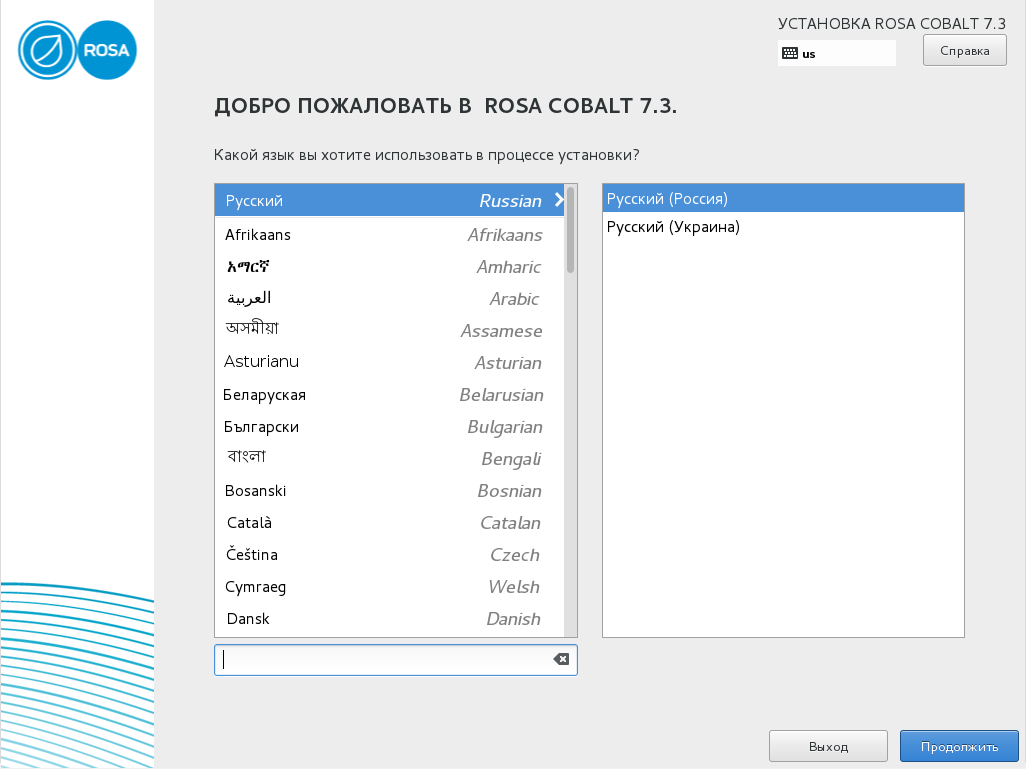
\includegraphics[scale=0.6]{0001.png}
\centering
\caption{Окно приложения TextMaker}
\end{figure}

 
 

Б\'{o}льшая 

\textbackslash
$\sim$ and \texttildelow from the textcomp package  %льда

\begin{center}
\begin{tabular}{ | m{15cm} | }
\hline
ООО «Любовь и голуби»,  оборудование для аквариумов — г.Рыбокочинск, ул.Капитана Врунгеля, дом 2\\
\hline
\end{tabular}
\end{center}


\textsc{текст капителью}

\textsuperscript{2}


\textsubscript{2}


{\footnotesize маленький шрифт}

% иерархический список
\begin{enumerate}
  \item Topic
  \begin{enumerate}[label*=\arabic*.]
    \item First Subtopic
    \item Second Subtopic
    \begin{enumerate}[label*=\arabic*.]
      \item First Sub-Subtopic
      \item Second Sub-Subtopic
    \end{enumerate}
  \end{enumerate}
\end{enumerate}


\begin{mdframed}[backgroundcolor=pink!50]
\textbf{\textit{FreeOffice}:} этот функционал отсутствует в \textbf{SoftMaker \textit{FreeOffice}}.
\end{mdframed}


\begin{center}
\begin{tabular}{  m{4cm}  m{12cm}  }
 \textbf{} & \textbf{}\\ 
 \hline
  \textbf{} & \\
  \textbf{} & \\ 
\textbf{} & \\
\textbf{} & \\
\end{tabular}
\end{center}
